% !Mode:: "TeX:DE:UTF-8:Main"
%\documentclass[handout]{beamer}
\documentclass{beamer}\usepackage[]{graphicx}\usepackage[]{color}
%% maxwidth is the original width if it is less than linewidth
%% otherwise use linewidth (to make sure the graphics do not exceed the margin)
\makeatletter
\def\maxwidth{ %
  \ifdim\Gin@nat@width>\linewidth
    \linewidth
  \else
    \Gin@nat@width
  \fi
}
\makeatother

\definecolor{fgcolor}{rgb}{0.345, 0.345, 0.345}
\newcommand{\hlnum}[1]{\textcolor[rgb]{0.686,0.059,0.569}{#1}}%
\newcommand{\hlstr}[1]{\textcolor[rgb]{0.192,0.494,0.8}{#1}}%
\newcommand{\hlcom}[1]{\textcolor[rgb]{0.678,0.584,0.686}{\textit{#1}}}%
\newcommand{\hlopt}[1]{\textcolor[rgb]{0,0,0}{#1}}%
\newcommand{\hlstd}[1]{\textcolor[rgb]{0.345,0.345,0.345}{#1}}%
\newcommand{\hlkwa}[1]{\textcolor[rgb]{0.161,0.373,0.58}{\textbf{#1}}}%
\newcommand{\hlkwb}[1]{\textcolor[rgb]{0.69,0.353,0.396}{#1}}%
\newcommand{\hlkwc}[1]{\textcolor[rgb]{0.333,0.667,0.333}{#1}}%
\newcommand{\hlkwd}[1]{\textcolor[rgb]{0.737,0.353,0.396}{\textbf{#1}}}%
\let\hlipl\hlkwb

\usepackage{framed}
\makeatletter
\newenvironment{kframe}{%
 \def\at@end@of@kframe{}%
 \ifinner\ifhmode%
  \def\at@end@of@kframe{\end{minipage}}%
  \begin{minipage}{\columnwidth}%
 \fi\fi%
 \def\FrameCommand##1{\hskip\@totalleftmargin \hskip-\fboxsep
 \colorbox{shadecolor}{##1}\hskip-\fboxsep
     % There is no \\@totalrightmargin, so:
     \hskip-\linewidth \hskip-\@totalleftmargin \hskip\columnwidth}%
 \MakeFramed {\advance\hsize-\width
   \@totalleftmargin\z@ \linewidth\hsize
   \@setminipage}}%
 {\par\unskip\endMakeFramed%
 \at@end@of@kframe}
\makeatother

\definecolor{shadecolor}{rgb}{.97, .97, .97}
\definecolor{messagecolor}{rgb}{0, 0, 0}
\definecolor{warningcolor}{rgb}{1, 0, 1}
\definecolor{errorcolor}{rgb}{1, 0, 0}
\newenvironment{knitrout}{}{} % an empty environment to be redefined in TeX

\usepackage{alltt}
\usepackage{tikz}
\usepackage[english]{babel}
\usepackage[utf8]{inputenc}
\usepackage[T1]{fontenc}
\usepackage{lipsum}

\usepackage{textpos} 
\usepackage{hyperref}
\usepackage{amsmath,amsthm,amsfonts,nicefrac,mathabx,amssymb}
\usepackage[subnum]{cases}
\usepackage{calligra, mathrsfs}
%\usepackage{natbib}
\usepackage{booktabs}
%\bibpunct{(}{)}{;}{a}{,}{,}

\usepackage{helvet}
\usepackage{graphicx}
\usepackage{color}
\usepackage{multirow,dcolumn}
\usepackage{ragged2e}
\usepackage{xcolor}
\usepackage{colortbl}
\usepackage{booktabs}
\usepackage{url}
\usepackage{bibentry}
\usepackage{chngcntr}

\usepackage{animate} %for animation

\usetheme{Gesis}


\newcommand{\eqname}[1]{\tag*{#1}} %equation title

%new math cal fonds
\newenvironment{frcseries}{\fontfamily{frc}\selectfont}{}
\newcommand{\textfrc}[1]{{\frcseries#1}}
\newcommand{\mathfrc}[1]{\text{\textfrc{#1}}}

\setcounter{tocdepth}{1}
\setbeamercolor*{section in toc}{fg=hellgrau}
\setbeamertemplate{bibliography item}[default]


\setcounter{secnumdepth}{3}
\setcounter{tocdepth}{3}


\newcommand{\E}[1]{\text{E}\left(#1\right)}
\newcommand{\V}[1]{\text{V}\left(#1\right)}
\newcommand{\Vest}[1]{\widehat{\text{V}}\left(#1\right)}
\newcommand{\MSE}[1]{\text{MSE}\left(#1\right)}
\newcommand{\COV}[2]{\text{COV}\left(#1,\,#2\right)}

\newcommand{\RN}[1]{%
  \textup{\uppercase\expandafter{\romannumeral#1}}%
}


\makeatletter

%%%%%%%%%%%%%%%%%%%%%%%%%%%%%% LyX specific LaTeX commands.
\providecommand{\LyX}{\texorpdfstring%
  {L\kern-.1667em\lower.25em\hbox{Y}\kern-.125emX\@}
  {LyX}}

%%%%%%%%%%%%%%%%%%%%%%%%%%%%% Textclass specific LaTeX commands.
% this default might be overridden by plain title style
 \newcommand\makebeamertitle{\frame{\maketitle}}%
 % (ERT) argument for the TOC
 \AtBeginDocument{%
   \let\origtableofcontents=\tableofcontents
   \def\tableofcontents{\@ifnextchar[{\origtableofcontents}{\gobbletableofcontents}}
   \def\gobbletableofcontents#1{\origtableofcontents}
 }

% A Section Title Slides
\AtBeginSection{\frame{\sectionpage}}
\AtBeginSubsection{\frame{\subsectionpage}}


\title{Sample Theory}
\subtitle{Epidemiological Study Design and Statistical Methods}

\author{Stefan Zins - GESIS}
\date{12.12.2017}

% Gestaltungsvarianten
% Kopfbandfarbe "shaded" von weiß zu blau: 
% \setbeamertemplate{gesisheadband}[shaded]
% andere Farbwerte
% \gesisCIbluecolors % = Blau und Orange aus CI, Blau als heller Hintergrund
% \gesisCIcolors     % = Blau und Orange aus CI, Sand als heller Hintergrund



%
% knitr setup 
% ------------------------------------------------------------------------------   


\IfFileExists{upquote.sty}{\usepackage{upquote}}{}
\begin{document}

\gesismaketitle % erzeugt Titelseite

\begin{frame}%[t]
  \frametitle{Content}
  
  \begin{itemize}
  \item Inference
  \item Design Based Inference
  \item Sampling Designs
  \item Calibration Weights
  \end{itemize}


\emph{SamplignAndEstimation} on GitHub, branch sampling\_short:
\url{https://github.com/BernStZi/SamplingAndEstimation/tree/sampling_short}
\end{frame}


\begin{frame}{Motivation}
 \begin{itemize}
    \item<1,4> Did you ever work with sample data? 
    \item<2,4> What kind of analysis have you done with sample data?
    \item<3,4> What concerns did you have while applying your analytically methods?
  \end{itemize}
\end{frame}

\section{Inference}


\begin{frame}{Law of Large Numbers (LLN)}
Weak law of large numbers: 

Suppose $ \{ y_1{,}y_2{,}\,\ldots{,}\,y_k{,}\,\ldots{,}\,y_n \}$ is a sequence of i.i.d. random variables with mean $\mu$ and $\mu \neq \infty$ and $\mu \neq -\infty$. Then for $n \rightarrow \infty$ then we have:

$$
\bar{y} \xrightarrow{P} \mu
$$

If the LLN holds we can have unbiased estimates, as our estimates will converge in probability to their expected (true) value.
\end{frame}


\begin{frame}{LLN Demonstration}
\onslide*<1>{
Suppose all $y_k$ follow an exponential distribution with mean and variance equal to one. We take repeatedly a sample of size $50$. For each sample the sample mean is calculated. The mean of the sample means should converge towards the true mean of the distribution with increasing number of samples.
}
\onslide<2>{
\begin{knitrout}
\definecolor{shadecolor}{rgb}{0.969, 0.969, 0.969}\color{fgcolor}

{\centering 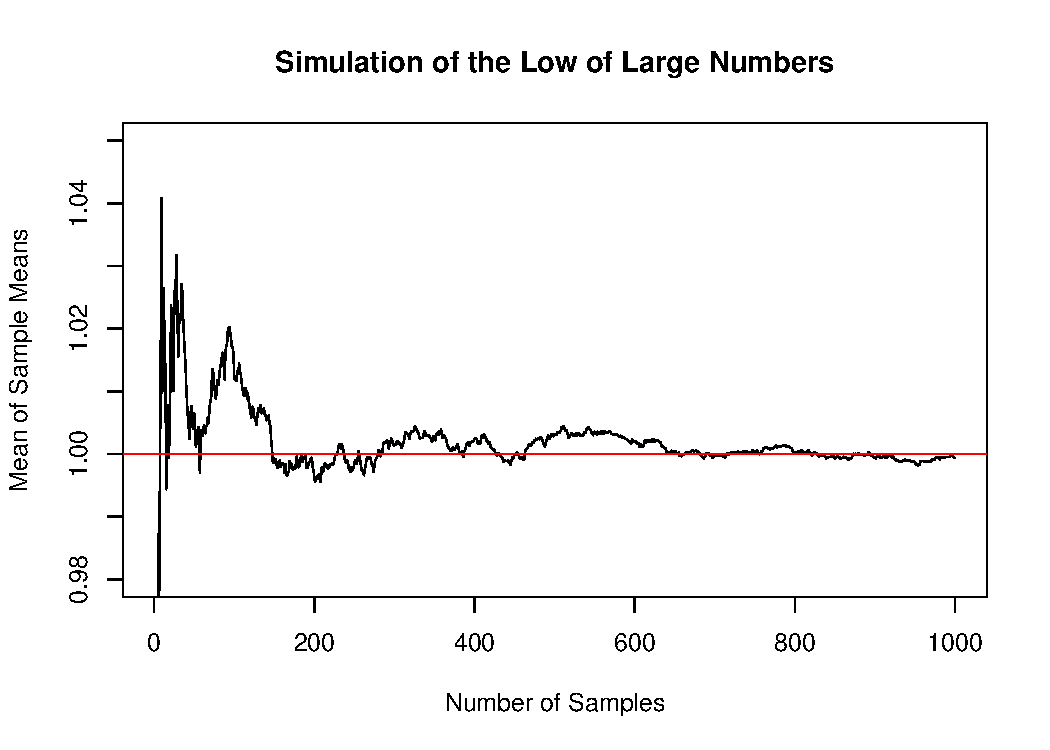
\includegraphics[width=.8\linewidth]{figure/LLN-1} 

}



\end{knitrout}
}
\end{frame}

\begin{frame}{Central  Limit Theorem (CLT)}
CLT of \emph{Lindeberg–L\'evy}: \\
Suppose $\{ y_1{,}y_2{,}\,\ldots{,}\,y_k{,}\,\ldots{,}\,y_N \}$ is a sequence of i.i.d. random variables with $V(y_i) = \sigma^2 < \infty\;\forall\; i=1,\,\ldots,\,N$. Then for $n \rightarrow \infty$ then we have:
$$
 \sqrt{n} ( \bar{y}- \mu )  \ {\xrightarrow {d}}\ N\left(0, \sigma^2 \right)
$$
If the CLT holds, symmetric confidence intervals can be constructed with quantiles from the standard normal distribution $\Phi(z)$
$$
\left[ \bar{y} + \Phi(\alpha/2)\sigma\sqrt{n} \,;\, \bar{y} + \Phi(1-\alpha/2)\sigma\sqrt{n}\right]
$$

%driven by sample size
\end{frame}


\begin{frame}{CLT Demonstration}



\onslide*<1>{
Suppose all $y_k$ follow an exponential distribution with mean and variance equal to one.
\begin{knitrout}
\definecolor{shadecolor}{rgb}{0.969, 0.969, 0.969}\color{fgcolor}

{\centering 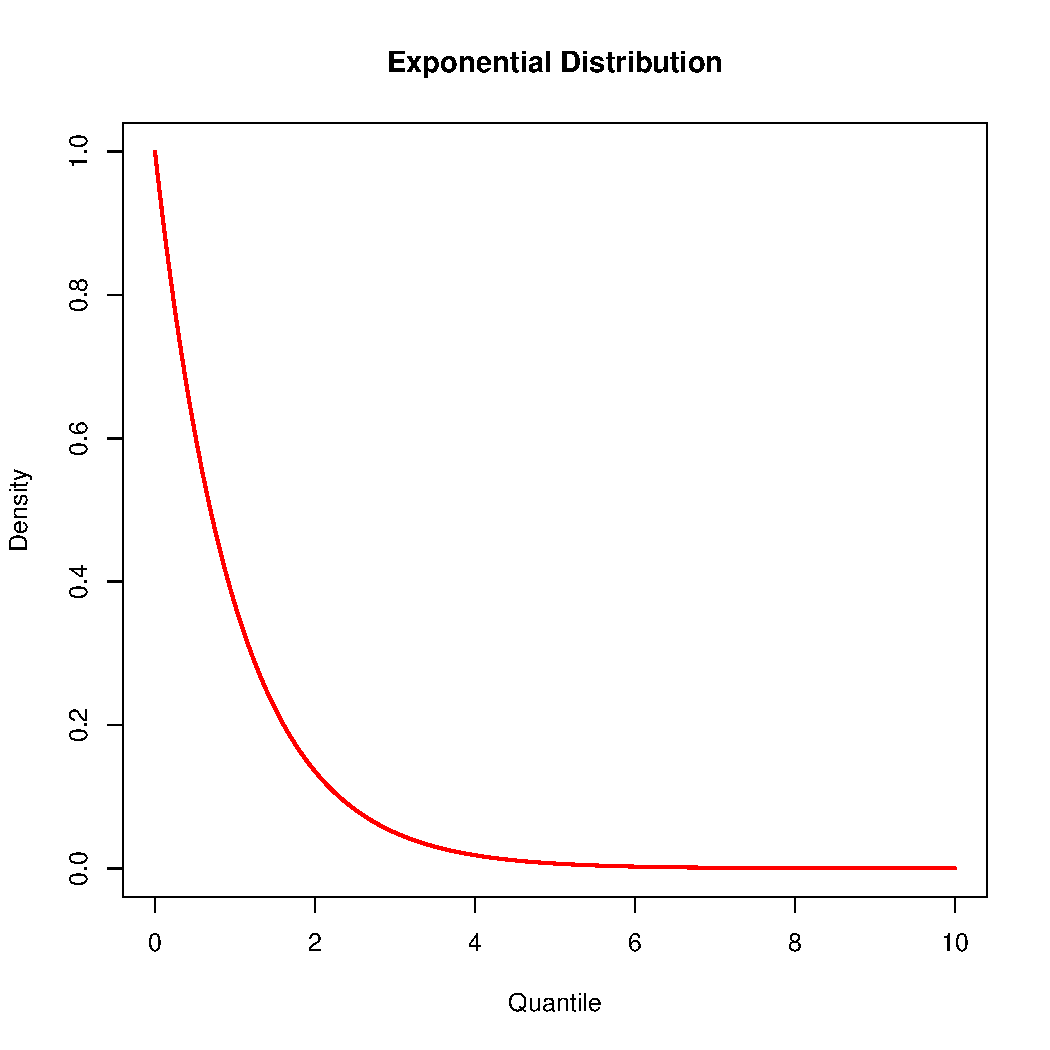
\includegraphics[width=\maxwidth,height=5cm]{figure/CLT_1-1} 

}



\end{knitrout}
}

\onslide*<2>{
\begin{knitrout}
\definecolor{shadecolor}{rgb}{0.969, 0.969, 0.969}\color{fgcolor}

{\centering 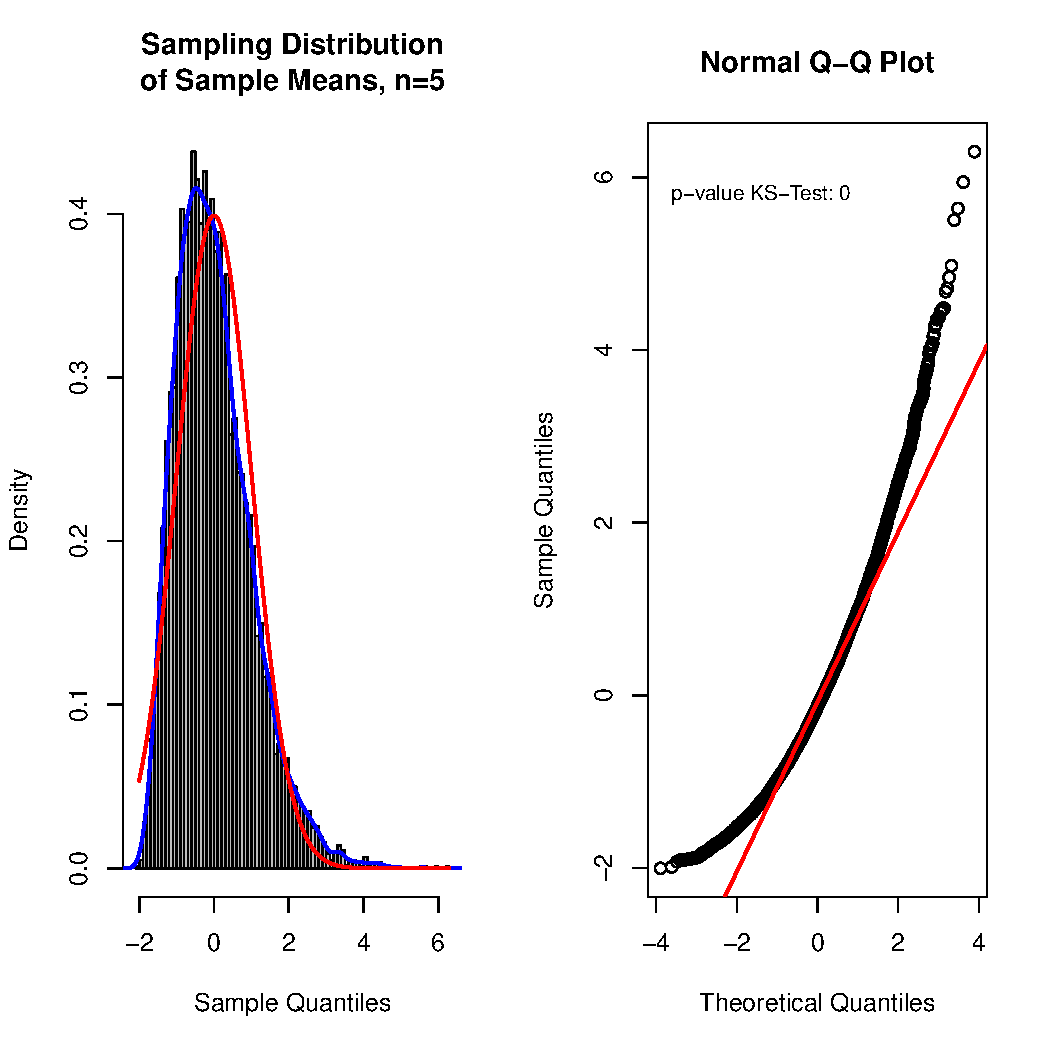
\includegraphics[width=\maxwidth,height=6.75cm]{figure/CLT_2-1} 

}



\end{knitrout}
 }

 \onslide*<3>{
\begin{knitrout}
\definecolor{shadecolor}{rgb}{0.969, 0.969, 0.969}\color{fgcolor}

{\centering 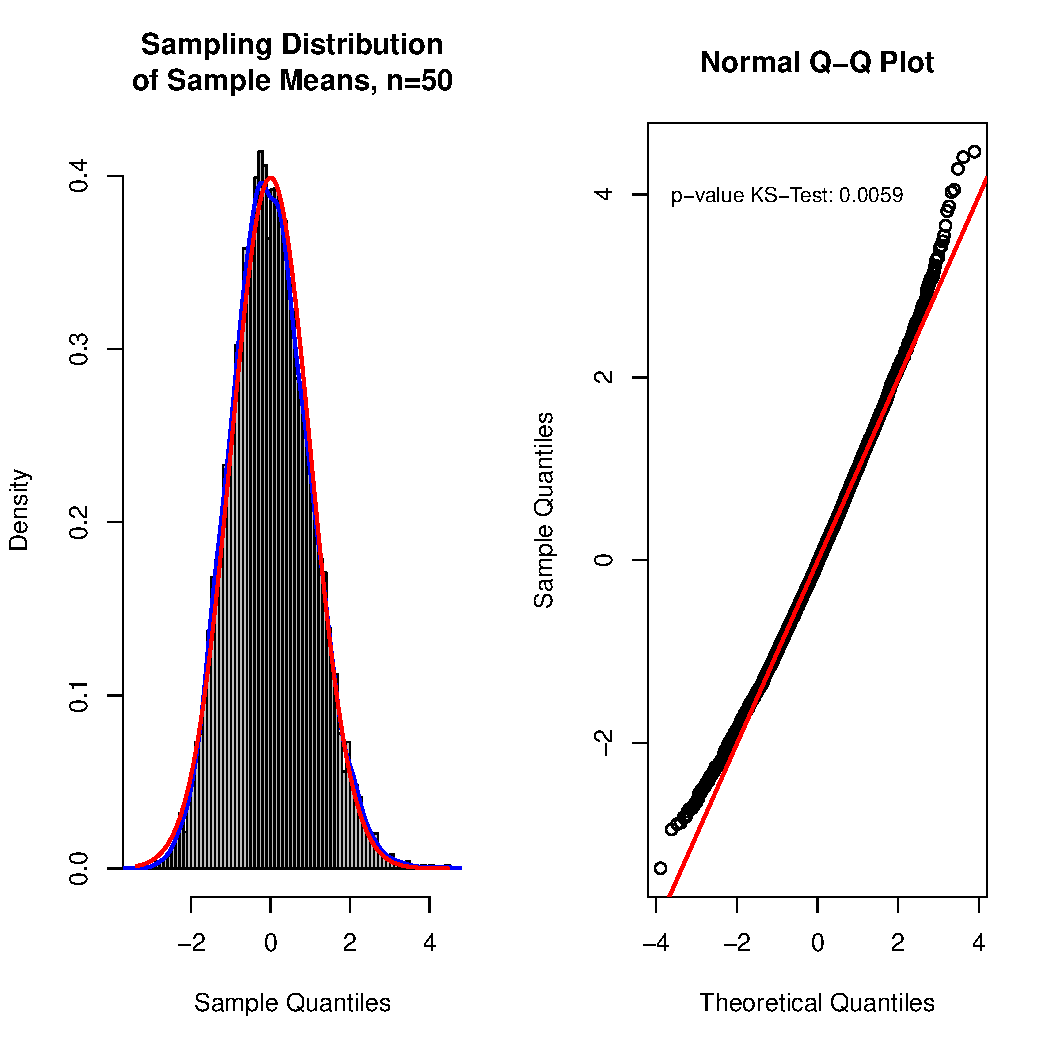
\includegraphics[width=\maxwidth,height=6.75cm]{figure/CLT_3-1} 

}



\end{knitrout}
 }

\onslide*<4>{
\begin{knitrout}
\definecolor{shadecolor}{rgb}{0.969, 0.969, 0.969}\color{fgcolor}

{\centering 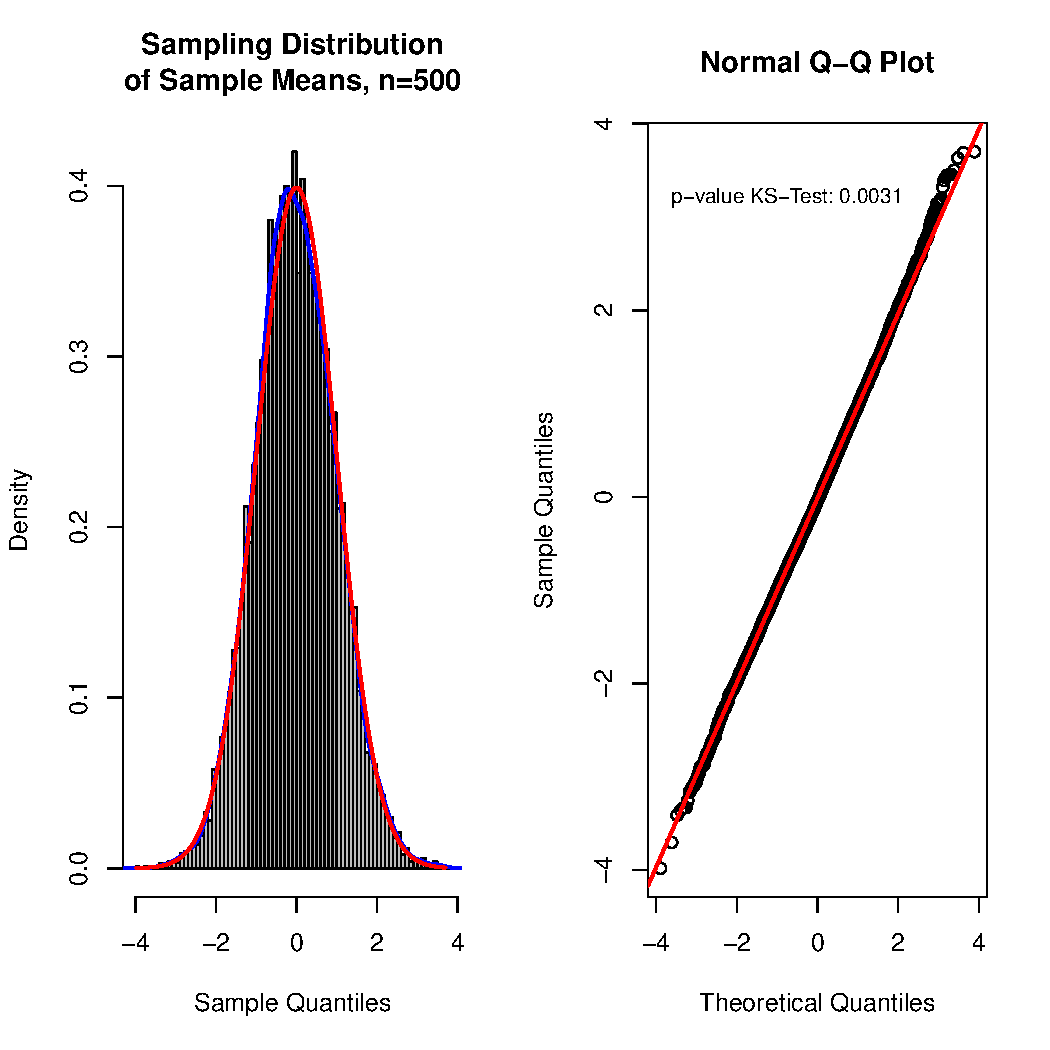
\includegraphics[width=\maxwidth,height=6.75cm]{figure/CLT_4-1} 

}



\end{knitrout}
}
\onslide*<5>{
\begin{knitrout}
\definecolor{shadecolor}{rgb}{0.969, 0.969, 0.969}\color{fgcolor}

{\centering 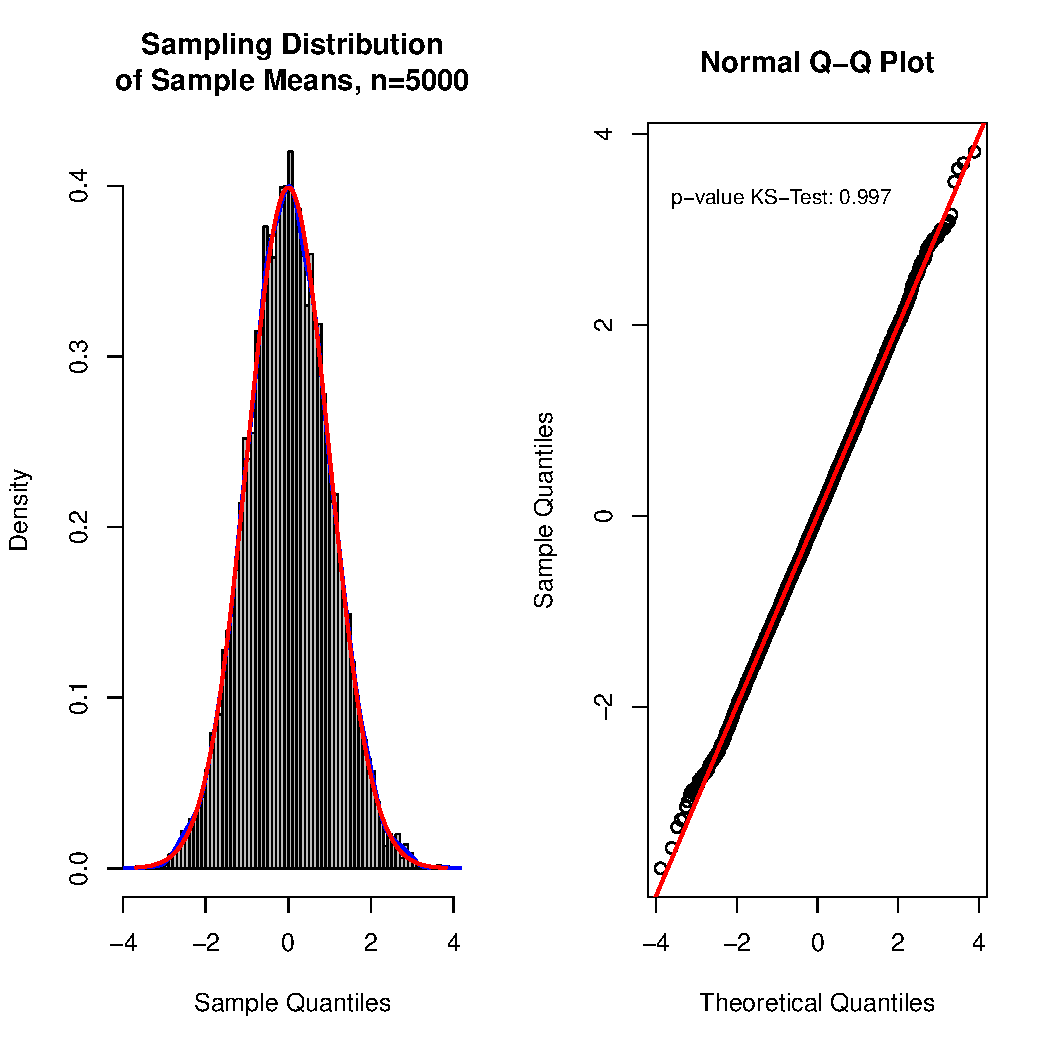
\includegraphics[width=\maxwidth,height=6.75cm]{figure/CLT_5-1} 

}



\end{knitrout}
}
\end{frame}



\section{Design Based Inference}


\begin{frame}{\alert{Finite} Population, Sample, and Sampling Design}

 \begin{itemize}
 \item[] 
 \begin{align}
 \mathcal{Y} = & \{ y_1{,}y_2{,}\,\ldots{,}\,y_k{,}\,\ldots{,}\,y_N \} \eqname{finite population of size $N$} \\
 \mathcal{U} = &\, \{ 1{,}2{,}\,\ldots{,}\,k{,}\,\ldots{,}\,N \} \eqname{sampling frame} \\
 \mathfrc{s} \subset &\, \mathcal{U} \eqname{sample of size $n$} \\
 \mathcal{P}(\mathcal{U}) & \eqname{all possible subsets of $\mathcal{U}$}
 \end{align}
 \item[] The discrete probability distribution $p(.)$ over $\mathcal{P}(\mathcal{U})$ is called a \emph{sampling design} and  $\mathcal{G}=\{ \mathfrc{s} | \mathfrc{s} \in \mathcal{P}(\mathcal{U}),\, p(\mathfrc{s}) > 0 \}$ is called the support of $p(.)$ with
$$
\sum_{\mathfrc{s} \in \mathcal{G}} p(\mathfrc{s}) = 1\;.
$$
 \end{itemize}
\end{frame}


\begin{frame}{Estimation}
\begin{align}
 \theta       & = f(\mathcal{Y})  \eqname{statistic of interest} \\
 \hat{\theta} & = f(\mathcal{Y}, \mathfrc{s} )  \eqname{estimator for $\theta$} \\
 \E{\hat{\theta}} & = \sum_{\mathfrc{s} \in \mathcal{G}} p(\mathfrc{s}) f(\mathcal{Y}, \mathfrc{s} )   \eqname{expected value of $\hat{\theta}$} \\
 \V{\hat{\theta}}   & =  \E{\hat{\theta}^2} -  {\E{\hat{\theta}}}^2 \eqname{variance of  $\hat{\theta}$} 
\end{align}
 $\E{.}$ and $\V{.}$ are always with respect to the sampling design $p(.)$ and
 an estimator is said to be unbiased if
 $$ \E{\hat{\theta}} = \theta\;. $$
\end{frame}


\begin{frame}{Inclusion Probabilities I}
\begin{align}
 I_k   &=   \begin{cases}   1  & \text{if}\; k \in \mathfrc{s} \\
                            0  & \text{else}  
          \end{cases}   \eqname{sampling indicator element $k$} \\
\E{I_k}     &  =   \pi_k    \eqname{inclusion probability of element $k$ } \\
\E{I_k I_l} &  =   \pi_{kl}  \eqname{joint expectation of $I_k$ and $I_l$} \\
\sum_{k \in \mathcal{U}}\pi_k & = \E{n} \eqname{expected sample size}
\end{align}

The $I_k$ are the \alert{only} random variables in the design based frame work and they follow a theoretical distribution, e.g. a \emph{Hypergeometric} distribution for SRS. 

\end{frame}


\begin{frame}{Inclusion Probabilities II}
With the inclusion probabilities design unbiased estimators can be constructed. For example an estimator for a total $\tau=\sum_{k \in \mathcal{U}} y_k$.
\begin{align*}
 \hat\tau &= \sum_{k \in \mathfrc{s}} \dfrac{y_k}{\pi_k} & \E{\hat\tau } &= \sum_{k \in \mathcal{U}} E(I_k) \dfrac{y_k}{\pi_k} = \tau
\end{align*}
$\pi_k^{-1}=d_k$ is also called the \alert{design weight} of element $k$.
% Many estimator can be written as functions of totals, which makes it possible to have at least design consistent estimtors for them.

$V(\hat\theta)=f(\mathcal{Y},\Sigma)$, with $\Sigma=(\E{I_k I_l}-\E{I_k} \E{I_l})_{k,l=1,\ldots,N}$.
For complex sampling designs $\Sigma$ can be very complex too and difficult to compute. In practice it is thus often unknown to data users. However there are approximations to $V(\hat\theta)$ that only require the $\pi_k$'s and are much simpler to estimate than $V(\hat\theta)$.

\end{frame}


\begin{frame}{Sample Mean with SRS}
  \small
  \begin{align*} 
  \mu = \dfrac{1}{N} \sum_{k \in \mathcal{U}}  y_k{,}  && \overline{y} = \sum_{k \in \mathfrc{s}}  \dfrac{y_k}{n}{,} && \sigma^2 = \dfrac{1}{N}\sum_{k \in \mathcal{U}} (y_k - \mu )^2{,}
  && V^2 = \sigma^2 \dfrac{N}{N-1}
  \end{align*}
  ~\\[-0.5cm]
  \begin{columns}[t]
   \onslide<2->{
    \begin{column}{.5\textwidth}
      \begin{align*} 
        \E{\overline{y}} & = \E{\sum_{k \in \mathcal{U}} I_k \dfrac{y_k}{n} } \\
        & = \dfrac{1}{n} \sum_{k \in \mathcal{U}} \E{I_k} y_k  \\
        & = \dfrac{1}{n} \sum_{k \in \mathcal{U}} \pi_k y_k  \\
        & = \dfrac{1}{N} \sum_{k \in \mathcal{U}}  y_k  
       \end{align*}
      \end{column}
    \begin{column}{.5\textwidth}
   }
   \onslide<3>{
      \begin{align*} 
        \V{\overline{y}} & = \V{\sum_{k \in \mathcal{U}} I_k \dfrac{y_k}{n}} \\
        & = \dfrac{1}{n^2} \sum_{k \in \mathcal{U}} \sum_{l \in \mathcal{U}} \COV{I_k}{I_l} y_k y_l  \\
        & = -\dfrac{1}{2} \dfrac{1}{n^2} \sum_{k \in \mathcal{U}} \sum_{l \in \mathcal{U}} (\pi_{kl}-\pi_k\pi_l)  \left(y_k - y_l \right)^2  \\
        & = \dfrac{N-n}{N-1} \dfrac{\sigma^2}{n}  =   \left( 1 -  \dfrac{n}{N} \right) \dfrac{V^2}{n}
      \end{align*}
    \end{column}
   }
    \end{columns}
 \end{frame}



\begin{frame}{Model-based Approach}
The sample data: $\{ y_1{,}y_2{,}\,\ldots{,}\,y_k{,}\,\ldots{,}\,y_n \}$, a sequence of i.i.d. random variables with
\begin{equation*}
  y_k \sim N(\mu, \sigma^2) \quad k=1\,\ldots,\,n{.}
\end{equation*}
~\\[-1cm]
\begin{columns}[t]
   \onslide<2->{
    \begin{column}{.5\textwidth}
      \begin{align*} 
        \E{\overline{y}}_{M} & = \E{\sum_{k \in \mathfrc{s}} \dfrac{y_k}{n} } \\
        & = \dfrac{1}{n} \sum_{k \in \mathfrc{s}} \mu  \\
        & = \mu
       \end{align*}
      \end{column}
    \begin{column}{.5\textwidth}
   }
   \onslide<3->{
      \begin{align*} 
        \V{\overline{y}}_{M} & = \V{\sum_{k \in \mathfrc{s}} \dfrac{y_k}{n}}_{M} \\
        & = \dfrac{1}{n^2} \sum_{k \in \mathfrc{s}} \sigma^2 \\
        & = \dfrac{\sigma^2}{n}    
      \end{align*}
    \end{column}
   }
    \end{columns}
     \onslide<4>{Note that there is no finite population correction.}
\end{frame}


\section{Sampling Designs}


\begin{frame}{Representative Sample}
\onslide*<1-2>{What is a representative sample? \newline}
\onslide*<2>{The popular concept of a representative sample it that the sample is a \emph{miniature} of the population.}

\onslide<3->{However, what do we actually want?}
\onslide<4->{\newline We want to estimate a statistic of interest with a certain level of precision.}
\onslide<5->{\newline The term \emph{representativ} does not come up in survey statistics}
\end{frame}

\begin{frame}{Elements of a Sampling Design}
\begin{itemize}
\item<1-> Sampling Frame(s)
 \begin{itemize}
  \item<1-> Access to the target population is of major importance for the selection of any sample
  \end{itemize}
\item<2-> Sampling Algorithm 
 \begin{itemize}
  \item<2-> A software implentation is needed
 \end{itemize}
\item<3-> Inklusion Probabilities
 \begin{itemize}
   \item<3-> $\pi_{k}>0   \; \forall\; k \in \mathcal{U}$
   \item<3-> $\pi_{kl}>0  \; \forall\; k \neq l \in \mathcal{U}$
 \end{itemize}
\end{itemize}
\end{frame}

\begin{frame}{Stratification}
A Population of 100 elements is stratified into $H=6$ strata.

%fig.keep='all',fig.show='asis'
\onslide*<1>{
\begin{knitrout}
\definecolor{shadecolor}{rgb}{0.969, 0.969, 0.969}\color{fgcolor}

{\centering 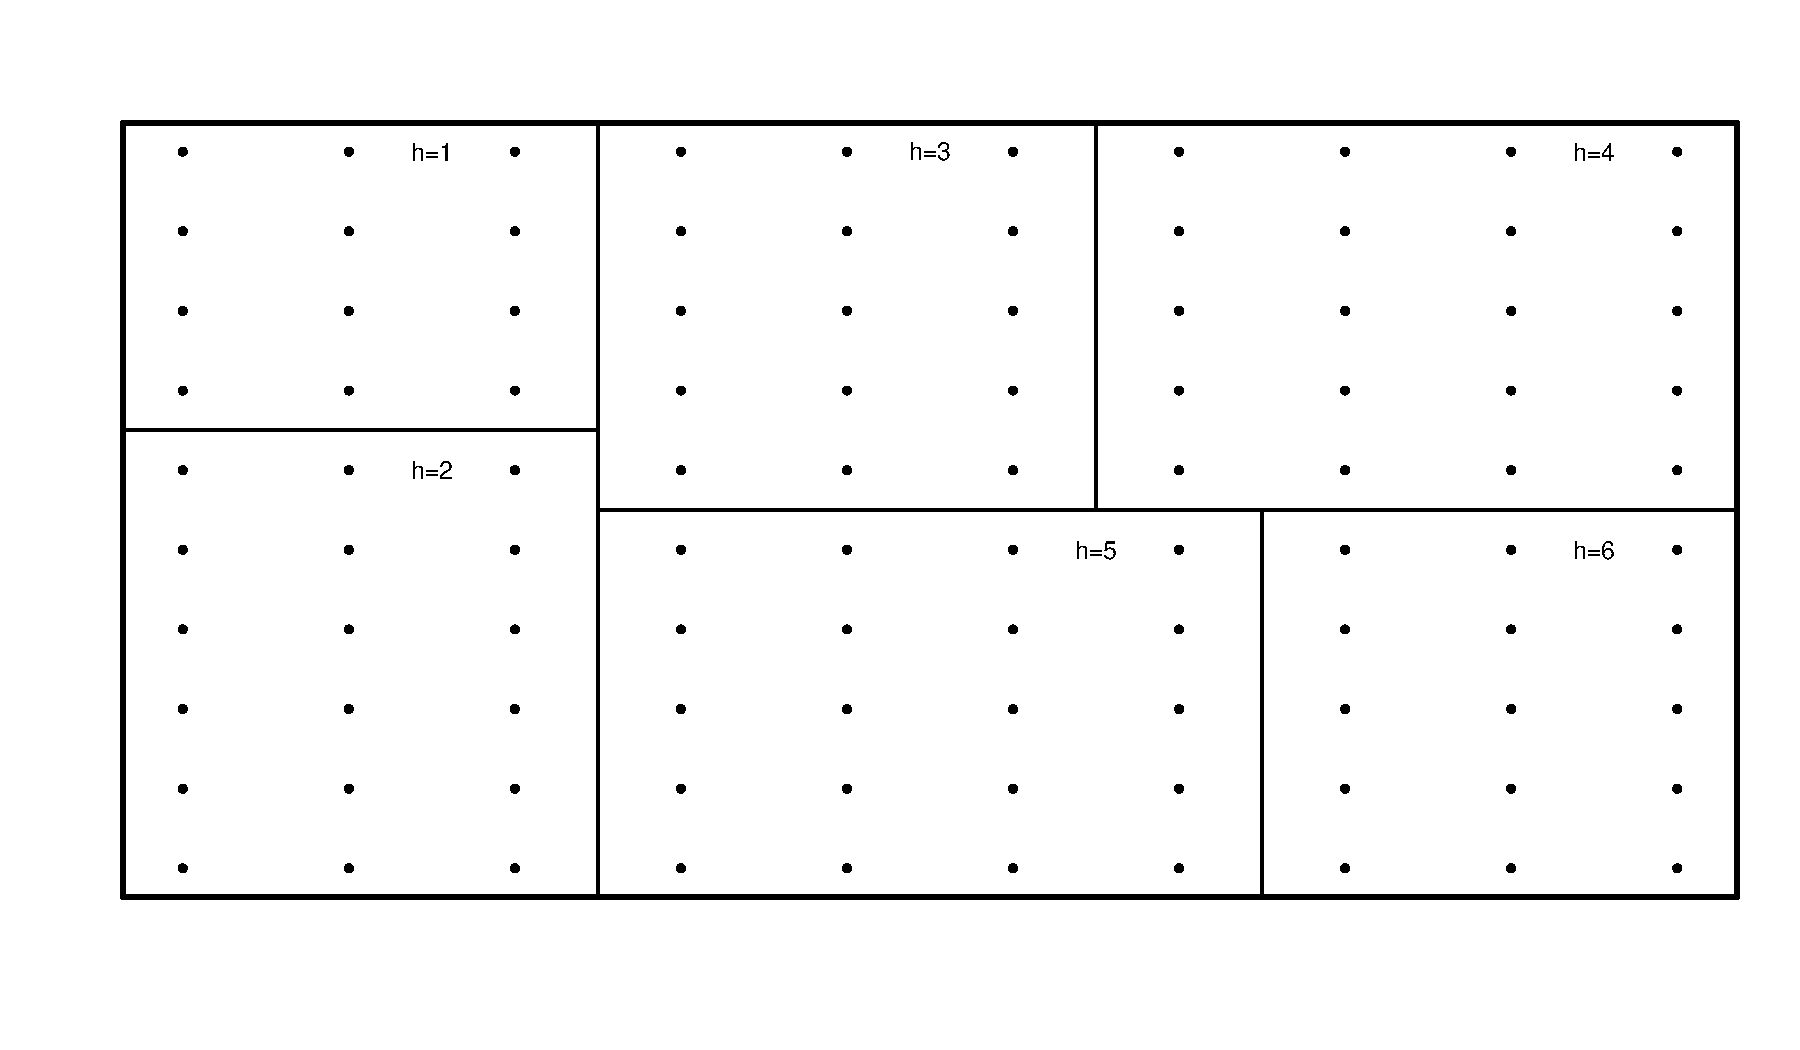
\includegraphics[width=.85\linewidth]{figure/StratPlot1-1} 

}



\end{knitrout}
}
\onslide<2>{
14 elements are selected population and their allocation is given by
\begin{tabular}{cccccc}
$n_1$ = 2  & $n_2$ = 3  & $n_3$ = 2  & $n_4$ = 3 & 
 $n_5$ = 3&  $n_6$ = 2\\
\end{tabular}

\begin{knitrout}
\definecolor{shadecolor}{rgb}{0.969, 0.969, 0.969}\color{fgcolor}

{\centering 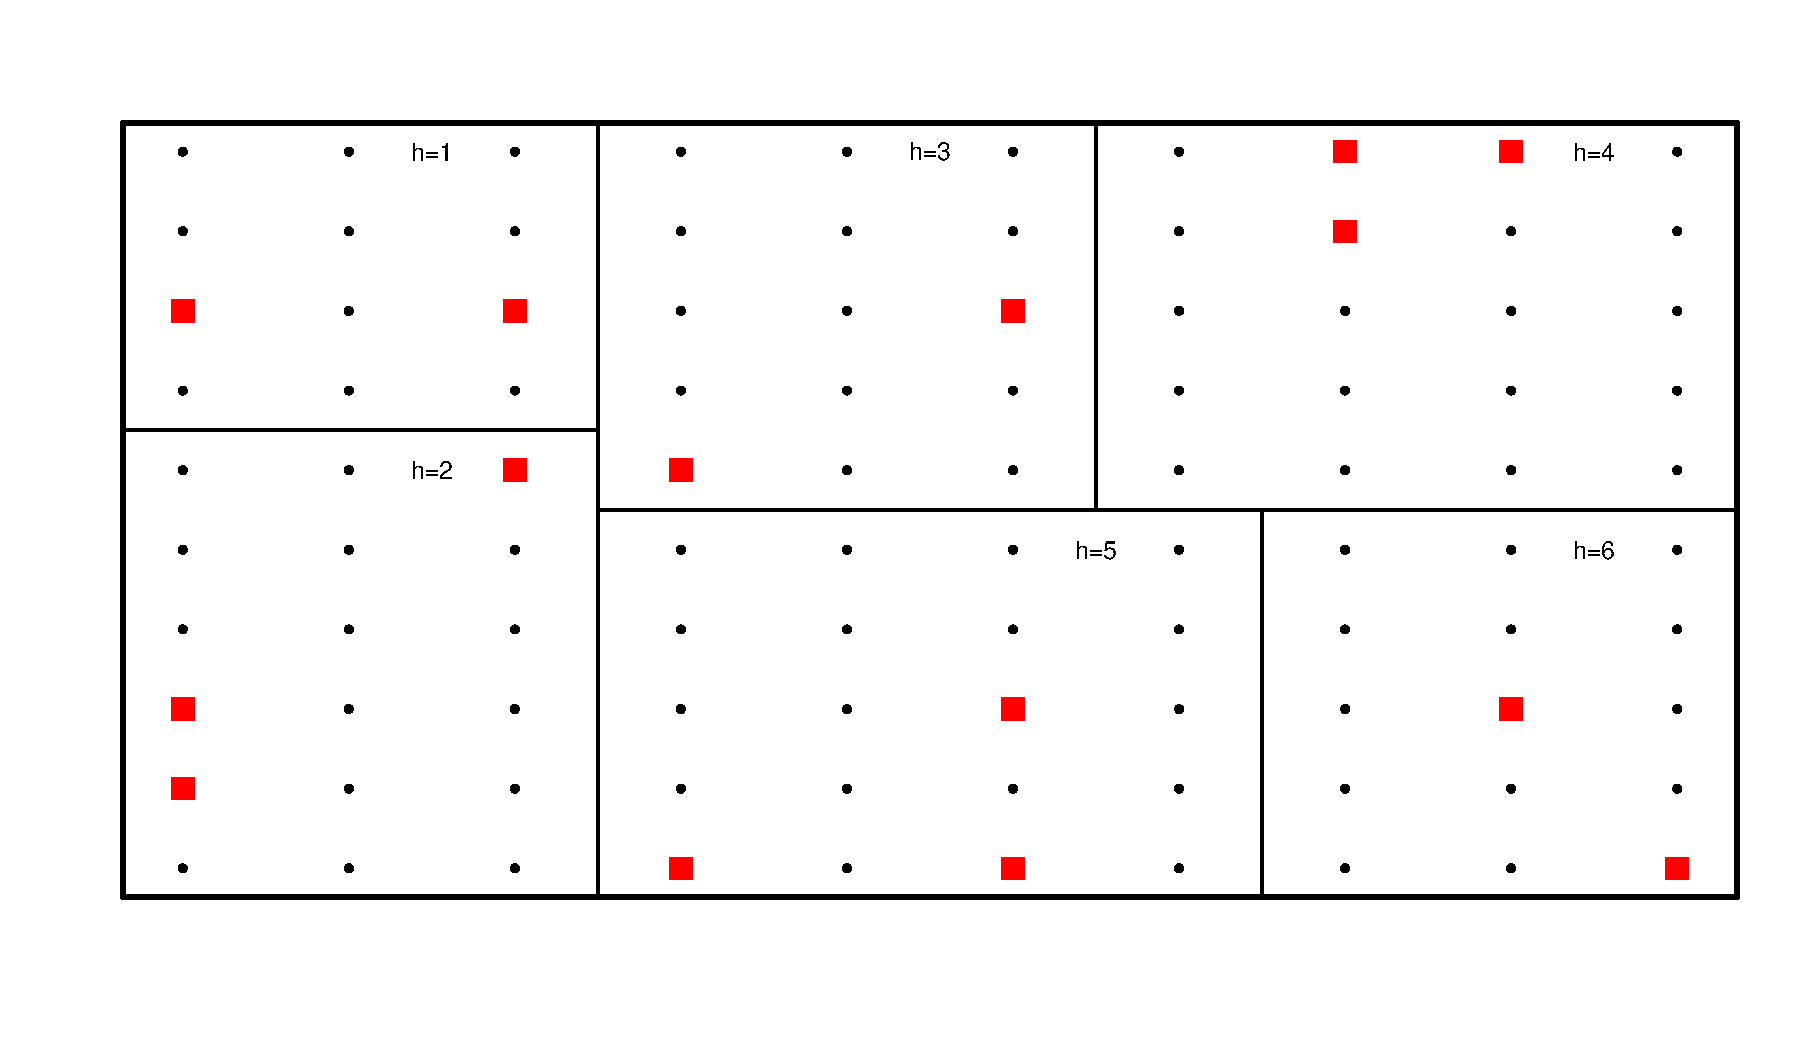
\includegraphics[width=.85\linewidth]{figure/StratPlot2-1} 

}



\end{knitrout}
}
\end{frame}


% \begin{frame}{Issues with Stratification}
% \begin{itemize}
% \item<1-> Why should stratification be used?
% \begin{itemize}
% \item<2-> To reduce the sampling variance of estimators.
% \item<2-> Sometimes it is necessary because of organizational reasons, (e.g. no joint sampling frame).
% \end{itemize}
% \item<3-> How should the population be stratified?
% \begin{itemize}
% \item<4-> A \emph{good} set of variables needs to be found for stratification.
% \item<4-> The number of strata has to be decided.
% \end{itemize}
% \item<5-> How should the overall sample size be allocated to the strata?
% \begin{itemize}
% \item<6-> Achieve proportionality between sample and population (i.e. the frame)
% \item<6-> Fulfill precision constraints for certain estimation domains
% \end{itemize}
% \end{itemize}
% 
% \end{frame}

\begin{frame}{Defining the Strata}
  \begin{table}\caption{Population ANOVA}
  \begin{tabular}{l | l | l }
  Source & df & Sum of Squares  \\
  \hline
   Between strata         & $H-1$ & $\text{SSB}  = \sum_{h=1}^H N_h ( \mu_{h} - \mu  )^2$  \\
   Within  strata         & $N-H$ & $\text{SSW}  = \sum_{h=1}^H (N_h-1) V_{h}^2$  \\
   Total,  about  $\mu_y$ & $N-1$ & $\text{SSTO} = (N-1) V^2$ \\
  \end{tabular}
  \end{table}
Stratification can reduce the sampling variance of estimators. The more homogeneous the strata are the higher is the gain in efficiency from using a stratified sample sample instead of SRS. That is if the SSW (variance within) is
considerably smaller that than the SSB (variance between). 
\end{frame}

\begin{frame}{Allocation Methods}
For all $h = 1{,}\,\ldots{,}\,H$
 \begin{equation*} \arraycolsep=1.4pt\def\arraystretch{2.2}
  n_h = \left\{ \begin{array}{l r}
        \dfrac{n}{H}  &\; \text{equal allocation} \\
        \dfrac{N_h}{N}  n    &\; \text{proportional allocation} \\
        \dfrac{N_h V_{h}}{\sum_{h=1}^H N_h V_{h} }  n  &\; \text{optimal allocation} 
  \end{array}\;\right.{,}
 \end{equation*}

Proportional allocation can also be done with respect to another variable, e.g. $\dfrac{\tau_h}{\tau}n$

% Variants of proportional allocation to totals
% proportional to y or auxiliar variable
% %the rounding probelem
\end{frame}

\begin{frame}[fragile]{Example Stratification}

\onslide*<1>{
We would like to estimate the difference in the mean Academic Performance Index (API) of all Californian schools between year 1999 and 2000 ($32.8$). To do that we select from all Californian schools two samples. One sample in 1999 and one in 2000. Both samples are selected by a  stratified (simple random) sample, where the Counties of California are used as the strata. The samples size for both samples is 205. From each County at least 2 schools are selected. The rest of the sampled size is allocated proportionally to the number of schools in the strata. The inclusion probability of a school in a particular stratum is the number of schools selected from that stratum divided by the total number of schools in that stratum. 
}
\onslide*<2>{
We use two estimator for variance estimation. One is design unbiased and the other is a naive estimator that uses no other design information than the design weights.

% latex table generated in R 3.5.0 by xtable 1.8-2 package
% Tue Dec 11 11:57:29 2018
\begin{table}[ht]
\centering
\begin{tabular}{rrrrr}
  \hline
 & Est & Vest & CI.lb & CI.ub \\ 
  \hline
Design & 24.07 & 231.501 & -5.754 & 53.888 \\ 
  Naive & 24.07 & 190.810 & -3.007 & 51.141 \\ 
   \hline
\end{tabular}
\end{table}


The stratification seems to be not very effective. So we construct 10 strata that are more homogeneous with regard to $\text{API}_{99}$ and $\text{API}_{00}$ (using \emph{k-means}) and select two new samples.

% latex table generated in R 3.5.0 by xtable 1.8-2 package
% Tue Dec 11 11:57:29 2018
\begin{table}[ht]
\centering
\begin{tabular}{rrrrr}
  \hline
 & Est & Vest & CI.lb & CI.ub \\ 
  \hline
Design & 33.24 & 4.879 & 28.916 & 37.574 \\ 
  Naive & 33.24 & 165.890 & 8.001 & 58.489 \\ 
   \hline
\end{tabular}
\end{table}

} 

\onslide*<3>{
We repeat the sampling with the better stratification 1000 times and compute the coverage rates for our confidence intervals.

% latex table generated in R 3.4.3 by xtable 1.8-2 package
% Sun Dec 10 19:11:40 2017
\begin{table}[ht]
\centering
\begin{tabular}{rrr}
  \hline
 & Design & Naive \\ 
  \hline
Coverage Rate & 0.965 & 1.000 \\ 
   \hline
\end{tabular}
\end{table}

}

\end{frame}

\begin{frame}{Clustering}

A Population of 100 elements is clustered into $N_{\RN{1}}=6$ cluster
%fig.keep='all',fig.show='asis'
\onslide*<1>{
\begin{knitrout}
\definecolor{shadecolor}{rgb}{0.969, 0.969, 0.969}\color{fgcolor}

{\centering 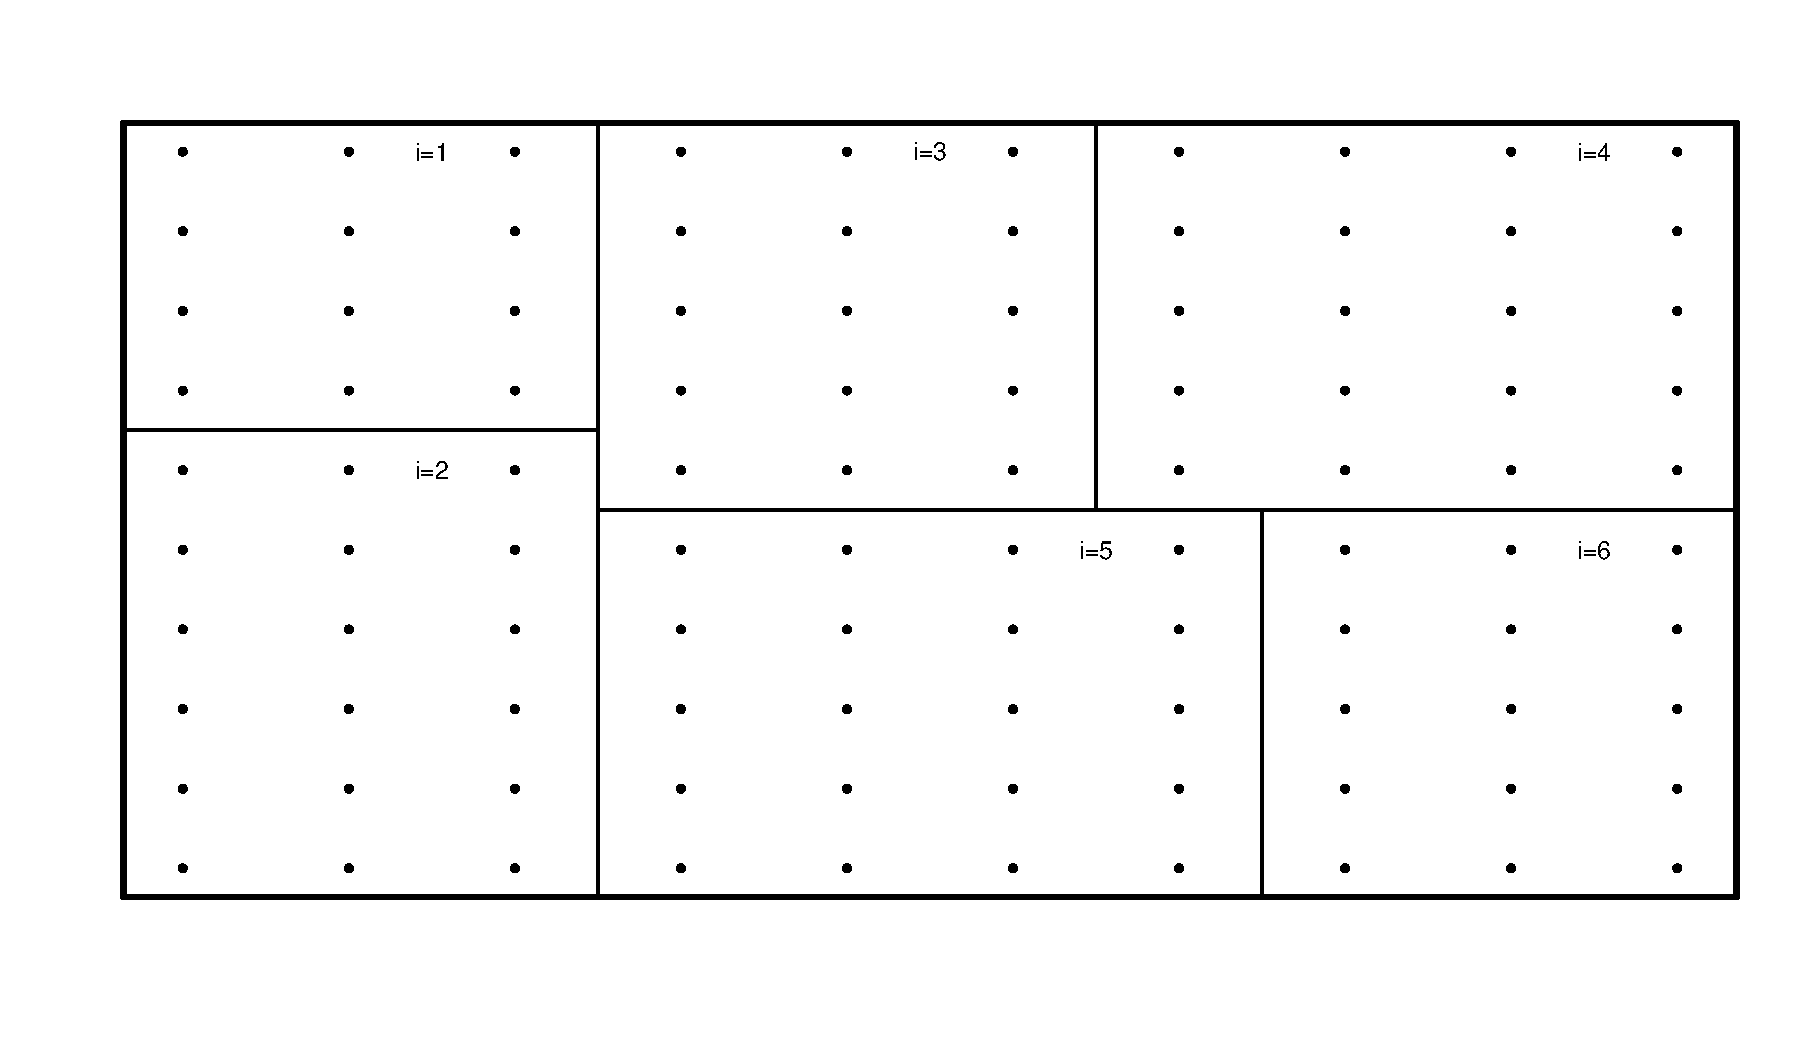
\includegraphics[width=.85\linewidth]{figure/CluPlot1-1} 

}



\end{knitrout}
}\onslide<2>{
and $n_{\RN{1}}=2$ clusters are selected from the population.
\begin{knitrout}
\definecolor{shadecolor}{rgb}{0.969, 0.969, 0.969}\color{fgcolor}

{\centering 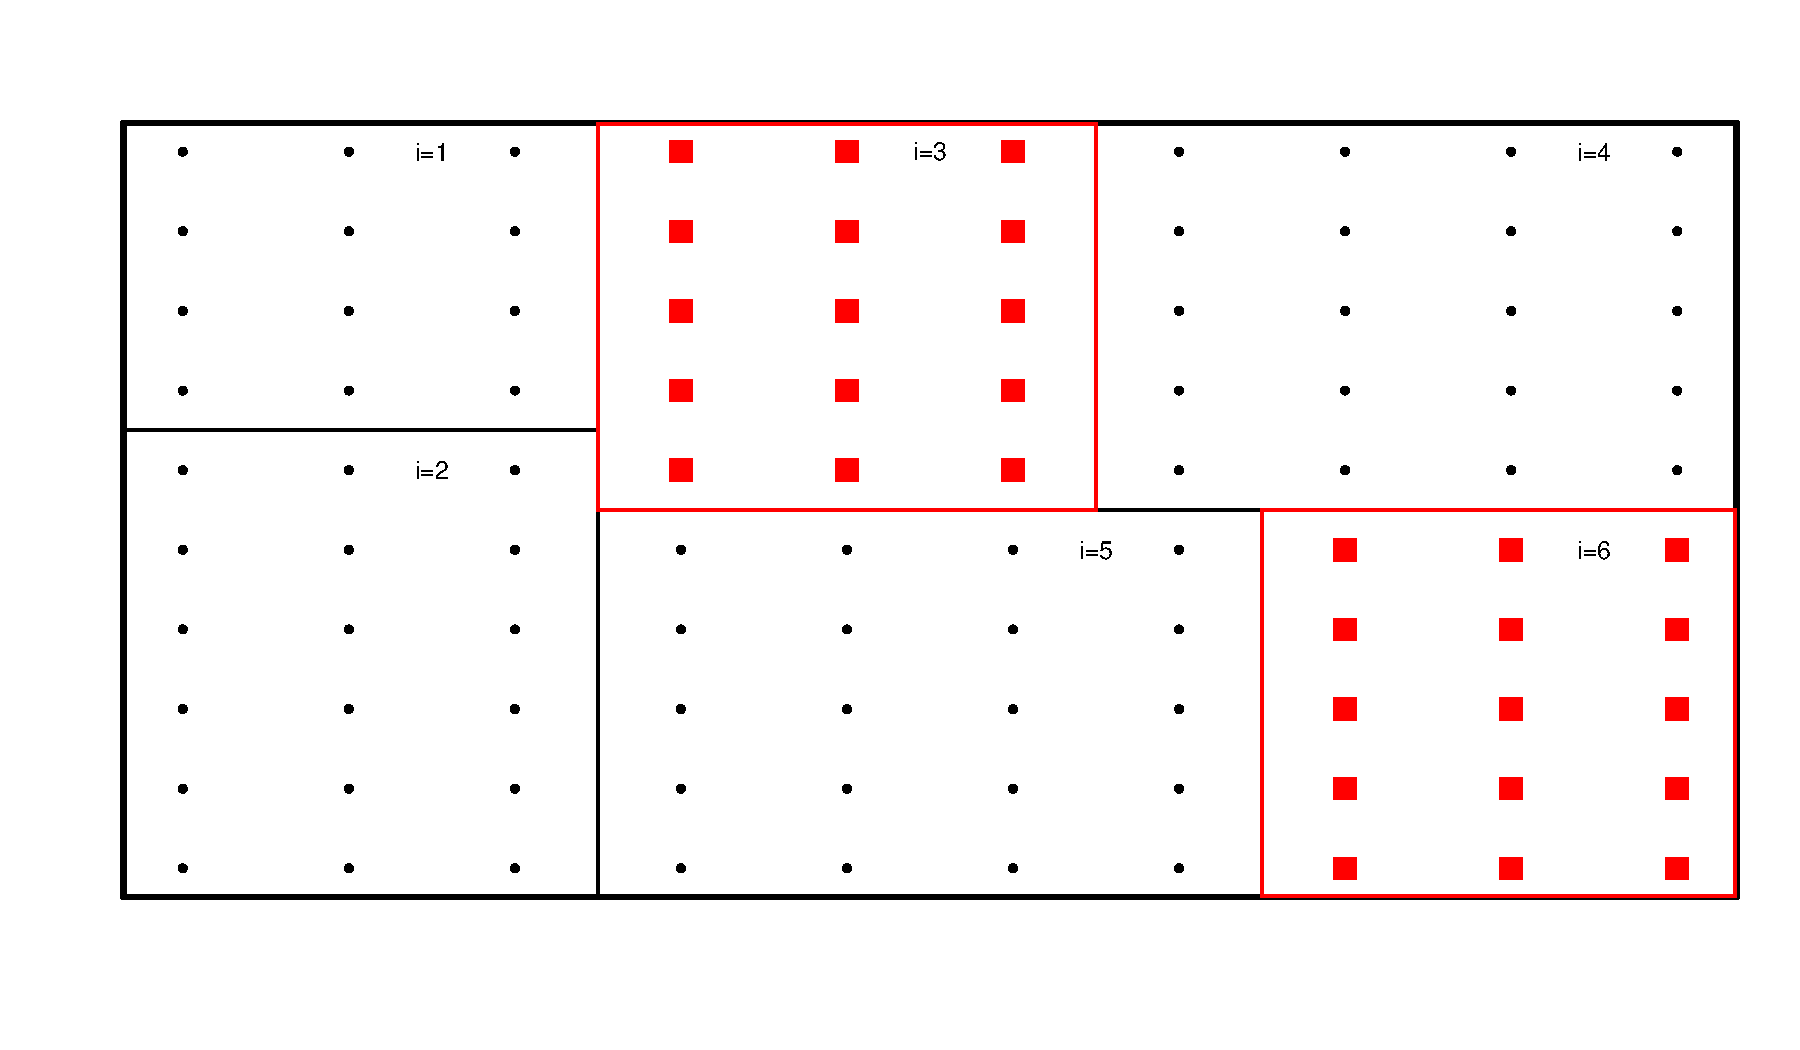
\includegraphics[width=.85\linewidth]{figure/CluPlot2-1} 

}



\end{knitrout}
}
\end{frame}


\begin{frame}{Cluster Sampling}
\onslide<1->{ Sampling elementary units is often not feasible (e.g. persons or businesses). Maybe there is no uniform sampling frame available to select them from, or it would be costly to do, because the selected elements would scatter to much over the a certain area and travel costs of interviewers would be to high. 
}
\onslide<2->{Thus, it is very common to select clusters, so called \emph{primary sampling units} (PSU's) that are populated by \emph{secondary sampling units} (SSU's).
}
\onslide<3->{Cluster sampling makes it still possible to obtain unbiased estimates but it can have a big influence on the variance. 
}
\onslide<4->{Compared to stratification cluster sampling tends to increase the sampling variance. What makes stratification efficient, a small within variance, has the opposite effect on cluster sampling.
}
\end{frame}



\begin{frame}[fragile]{Example Clustering}

\onslide*<1>{
Now we use for our Californian school survey cluster sampling. Both samples are selected by a (simple) cluster sample, where the clusters are the School Districts of California. 25 clusters are selected for both samples and the expected number of schools in each sample is $205$. Each cluster has the same inclusion probability, $0.0330251$ (25 divided by $757$, the number of clusters). 
}
\onslide*<2>{
We use two estimator for variance estimation. One is design unbiased and the other is a naive estimator that uses no other design information than the design weights.

% latex table generated in R 3.5.0 by xtable 1.8-2 package
% Tue Dec 11 11:57:29 2018
\begin{table}[ht]
\centering
\begin{tabular}{rrrrr}
  \hline
 & Est & Vest & CI.lb & CI.ub \\ 
  \hline
Design & 110.35 & 1755.376 & 28.229 & 192.463 \\ 
  Naive & 110.35 & 168.378 & 84.914 & 135.779 \\ 
   \hline
\end{tabular}
\end{table}


} 

\onslide*<3>{
We repeat the sampling 1000 times and compute the coverage rates for our confidence intervals.

% latex table generated in R 3.4.3 by xtable 1.8-2 package
% Sun Dec 10 19:29:37 2017
\begin{table}[ht]
\centering
\begin{tabular}{rrr}
  \hline
 & Design & Naive \\ 
  \hline
Coverage Rate & 0.863 & 0.415 \\ 
   \hline
\end{tabular}
\end{table}



Because of the under estimation by the naive variance estimator the naive approach results in a severe under coverage.
The design based approach does not under estimate the variance but their is a problem with the application of the CLT for building the confidence intervals.

}

\onslide*<4>{
We repeat the simulation, but only with 100 replications and this time we sample the clusters proportional to their number of schools. Thus the inclusion probability of each cluster is $\dfrac{N_i}{N}*25$, where $N_i$ is the number of schools in the $i$-th cluster and N the total number of schools ($6194$).

% latex table generated in R 3.4.3 by xtable 1.8-2 package
% Mon Dec 11 22:20:12 2017
\begin{table}[ht]
\centering
\begin{tabular}{rrr}
  \hline
 & Design & Naive \\ 
  \hline
Coverage Rate & 0.980 & 0.330 \\ 
   \hline
\end{tabular}
\end{table}

}

\end{frame}



%\section{Complex Sampling Designs - Two Stage Sampling}

\begin{frame}{Two Stage Sampling}
% A Population of 100 elements is clustered into $N_{\RN{1}}=6$ clusters
% and $n_{\RN{1}}=n_I$ clusters (PSU) are selected at the first sampling stage
\onslide*<1>{
\begin{knitrout}
\definecolor{shadecolor}{rgb}{0.969, 0.969, 0.969}\color{fgcolor}

{\centering 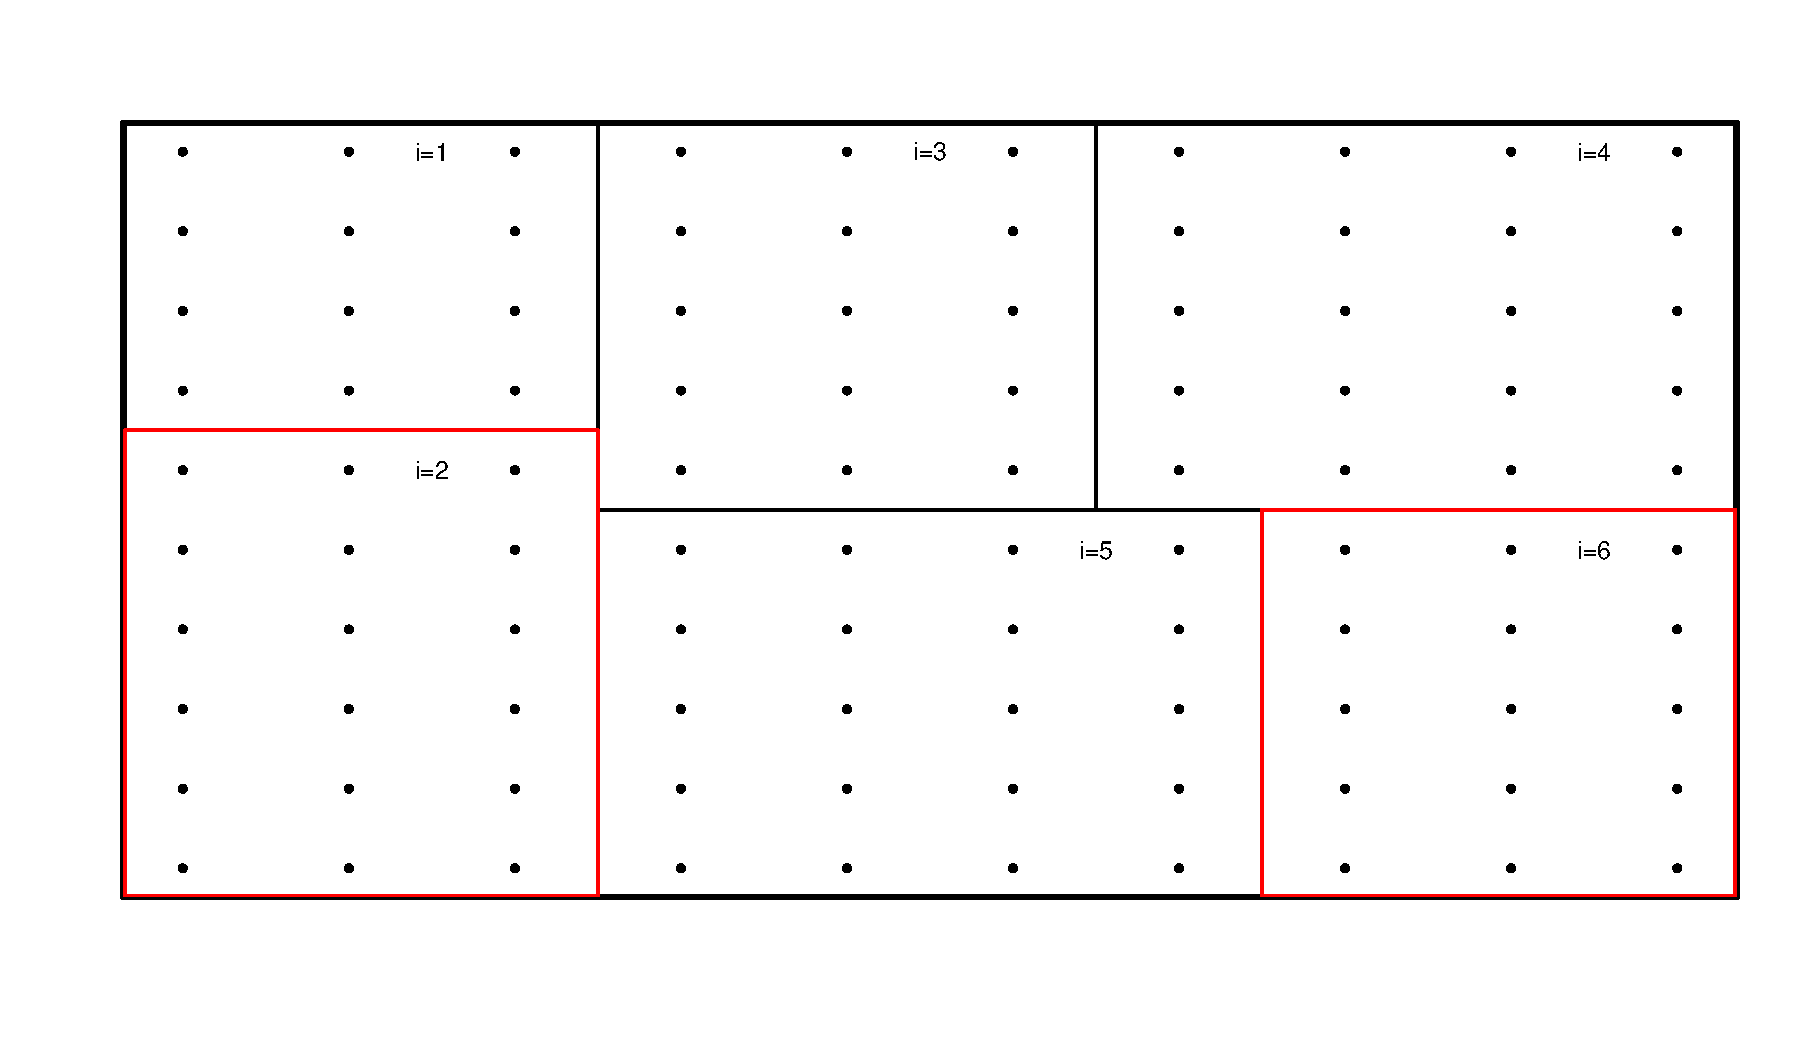
\includegraphics[width=.85\linewidth]{figure/CluPlot1_2-1} 

}



\end{knitrout}

}\onslide<2>{
and $n_{i}=4$ elements are selected from each sampled cluster.
\begin{knitrout}
\definecolor{shadecolor}{rgb}{0.969, 0.969, 0.969}\color{fgcolor}

{\centering 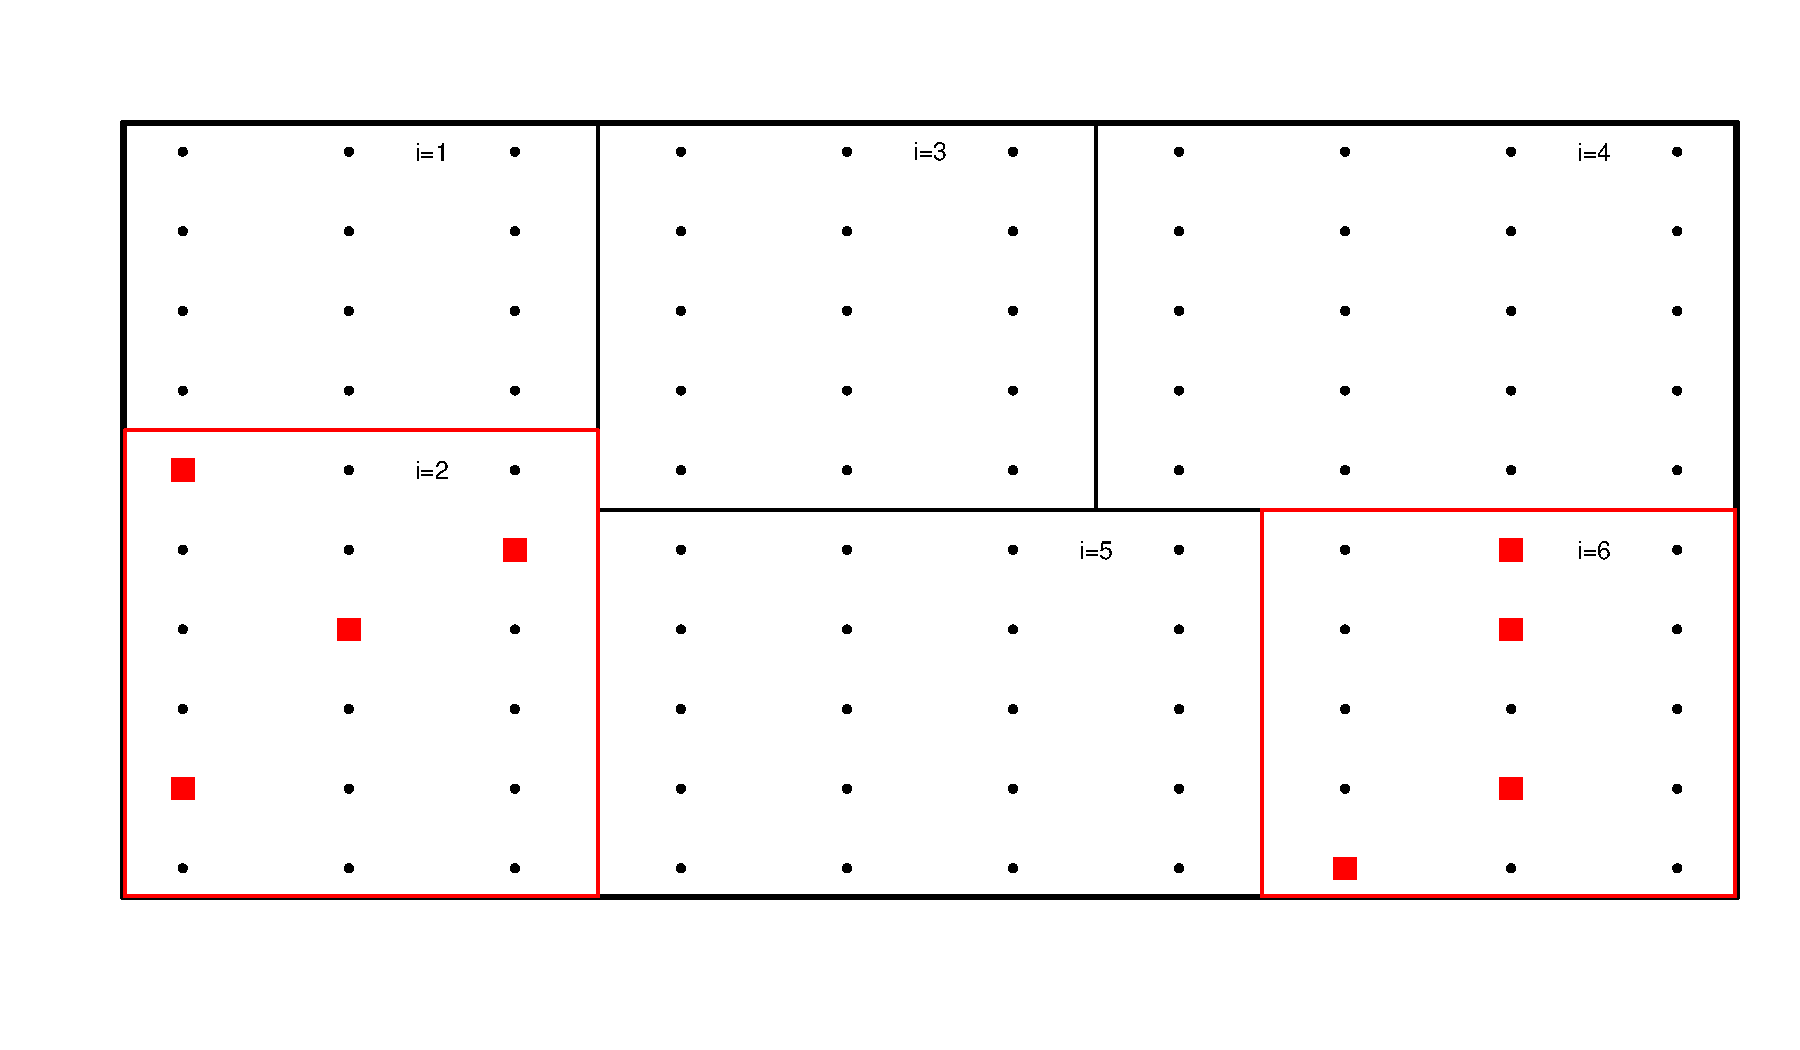
\includegraphics[width=.85\linewidth]{figure/CluPlot2_2-1} 

}



\end{knitrout}
}
\end{frame}


\section{Calibration Weights}

\begin{frame}{Calibrating Design Weights I}

\onslide*<1>{The general idea is to exploit the relationship between auxiliary variables and the variable of interest to improve the efficiency of estimators.}
\onslide*<2>{ The following problem is solved with weight calibration: \newline
For a give design $p(.)$ and a sample $\mathfrc{s}$ weights $w_k$ for all $k \in  \mathfrc{s}$ have to be found that minimize
 $$\sum_{k \in  \mathfrc{s} } G_k(w_k,d_k,c_k)\;,$$
subject to constraints
 $$
 \sum_{k \in \mathfrc{s} } w_k \mathbf{x}_k = \sum_{k \in \mathcal{U} } \mathbf{x}_k = \boldsymbol{\tau}_x
 $$
where $\mathbf{x}_k=(x_{k1},\,x_{k2},\,\ldots,\,x_{kQ})^\top$ is a vector of $q$ auxiliary variables for element $k$. $G_k$ is a measure of distance between $w_k$ and $d_k$ and $c_k$ is a factor that can be freely chosen for additional flexibility.
}
\end{frame}


\begin{frame}{Calibrating Design Weights II}
\onslide<1->{
The calibrated weight of element $k$ $w_k$ can be described as $w_k = d_k g_k$, where $g_k$ is the adjustment made to the design weight $d_k$.
The goal is the keep $g_k$ as close to one as possible, because the design weights 
have the desirable property to enable unbiased estimation.
}
\onslide<2->{
Common methods to compute calibration weights are:
}
\begin{itemize}
\item<3-> Post-stratification
\item<4-> Raking
\item<5-> General linear Calibration
\end{itemize}
\onslide<6->{
$$
g_k = 1 + \left(\Big(\sum_{k \in \mathcal{U} } \mathbf{x}_k - \sum_{k \in \mathfrc{s} } d_k \mathbf{x}_k\Big)^\top \Big(\sum_{k \in \mathfrc{s} } d_k c_k \mathbf{x}_k (\mathbf{x}_k)^\top \Big)^{-1}\right)^\top c_k \mathbf{x}_k
$$
}
\end{frame}





\begin{frame}{Example Calibration Weights}
Again we sample Californian schools from the API data set.

\begin{itemize}
\item Design: We take a sample schools 100 with $\pi_k$'s proportional to their size (i.e. number of students enrolled) and use stratification by school type (i.e. Elementary, Middle, or High School).
\item Calibration: As an auxiliary variable for calibration we use a classification of schools based of their $\text{API}_{99}$ and $\text{API}_{00}$ values (using \emph{k-means}).
\item Estimation: We are interested in estimating the mean value of $\text{API}_{00}$
\item Simulation: We repeat the sampling process $2500$ times to assess the bias of point estimates and the coverage rate of confidence intervals (CR)
\end{itemize}
\end{frame}

 
\begin{frame}[fragile]{Example Calibration Weights}
% latex table generated in R 3.5.0 by xtable 1.8-2 package
% Tue Dec 11 11:57:30 2018
\begin{table}[ht]
\centering
\caption{Expected Values of Point and Variance Estimators} 
\begin{tabular}{rrrrr}
  \hline
 & Naive & Design & Cal.Naive & Cal.Design \\ 
  \hline
Pest & 645.9028 & 664.7626 & 664.6393 & 664.6393 \\ 
  Vest & 12.8075 & 15.0301 & 15.3799 & 5.8138 \\ 
   \hline
\end{tabular}
\end{table}


% latex table generated in R 3.5.0 by xtable 1.8-2 package
% Tue Dec 11 11:57:30 2018
\begin{table}[ht]
\centering
\caption{Bias and Coverage Rates} 
\begin{tabular}{rrrrr}
  \hline
 & Naive & Design & Cal.Naive & Cal.Design \\ 
  \hline
Bias & -0.0284 & -0.0001 & -0.0002 & -0.0002 \\ 
  CR & 0.6828 & 0.9436 & 1.0000 & 0.9372 \\ 
   \hline
\end{tabular}
\end{table}


\end{frame}


% 
% 
% % 
% % 
% \begin{frame}{Two Stage Sampling}
%  \begin{description}
%  \item[First  stage] A sample $\mathfrc{s}_{\RN{1}}$ of PSU's is drawn from $\mathcal{U}_{\RN{1}}$ according to some sampling design $p_{\RN{1}}(.)$
%  \item[Second stage] For every $i \in \mathfrc{s}_{\RN{1}}$ a sample $\mathfrc{s}_i$ of SSU's is selected from $\mathcal{U}_i$ according to some design $p_i(.|\mathfrc{s}_{\RN{1}})$
%  \end{description}
%  The resulting sample of SSU's is denote $\mathfrc{s}= \bigcup_{i \in \mathfrc{s}_{\RN{1}}} \mathfrc{s}_i $.
%  In general, samples $\mathfrc{s}_i$ are selected independently of each other, thus, the inclusion probability of a element $k \in \mathcal{U}_i$ is
% $$\pi_k=\pi_{\RN{1}i}\pi_{k|i}\;,$$
% where $\pi_{\RN{1}i}$ is the probability of selecting the $i$-th PSU and $\pi_{k|i}$  the probability of selecting
% the $k$-th SSU within the $i$-th PSU.
% \end{frame}
% 
% 
% 
% \begin{frame}[fragile]{Example Two Stage Sampling}
% <<TwoStageExam, echo=FALSE, cache=FASLE, results='hide', warning=FALSE, message=FALSE, cache=TRUE>>=
% set.seed(2251)
% data(api)
% 
% select.apiTwoStage <- 
%   function(n_I, n_c){
%     dat <- apipop
%     h_c  <- table(dat$cnum)/nrow(dat)*n_I
%     
%     
%     p_c  <- h_c%%1
%     d_c  <- h_c%/%1
%     s_c  <- UPmaxentropy(p_c)
%     
%     n_i  <- (s_c+d_c)*n_c
%     
%     s.snum <- unlist(
%       mapply(function(x,y) sample(as.character(x), y), 
%              tapply(dat$snum,dat$cnum,identity)[names(n_i)],
%              n_i
%       )
%     )
%     
%     h_ci  <- h_c[as.character(dat$cnum)]
%     n_i.m <- rep(n_c,length(h_ci))
%     
%     n_i.m[h_ci>1] <- h_ci[h_ci>1]*n_c
%     
%     p_ci         <- h_ci
%     p_ci[h_ci>1] <- 1
%     
%     dat$fpc2 <- n_i.m[dat$cnum]/table(dat$cnum)[as.character(dat$cnum)]
%     dat$fpc1 <- p_ci[as.character(dat$cnum)]
%     
%     
%     apiclus3 <- dat[dat$snum%in%as.numeric(s.snum),]
%     
%     svydesign(id=~cnum+snum, fpc = ~fpc1 + fpc2, data=apiclus3, pps = "brewer")
%     
%     
%     
%   }
% 
% dmultstag_1 <- select.apiTwoStage(25,2)
% 
% sum.lm.naive <- summary(lm(api00~ell+meals+mobility+stype, 
%                            data = dmultstag_1$variables, 
%                            weights = weights(dmultstag_1)))
% 
% sum.lm.svy   <- summary(svyglm(api00~ell+meals+mobility+stype, 
%                                design=dmultstag_1))
% 
% @
% \onslide*<1>{
% For our Californian schools would like to estimate the following model $\text{API}_{00} = \text{ell}+\text{meals}+\text{mobility}+\text{stype}$,
% where
% \begin{itemize}
% \item[ell] = English Language Learners (percent)
% \item[meals] =  Percentage of students eligible for subsidized meals,
% \item[mobility] = percentage of students for whom this is the first year at the school,
% \item[stype] = Elementary/Middle/High School
% \end{itemize}
% Now we use a two stage sample. As PSUs the counties of California are used, the SSU are the schools. 25 PSUs are selected with probablity proportional to their number of schools. Within each selected PSU 2 schools are sampled by a SRS.
%  }
% \onslide<2>{
% 
% <<TwoStageRes,  echo=FALSE, cache=FALSE, results='asis'>>=
% tab.naive<-xtable(sum.lm.naive,digits = c(0,3,3,3,3),caption = "Naive")
% tab.svy  <- xtable(sum.lm.svy,digits = c(0,3,3,3,3),caption = "Design")
% 
% print(tab.naive, scalebox=0.6,caption.placement='top')
% print(tab.svy, scalebox=0.6,caption.placement='top')
% @
% }
% \end{frame}
% 

% \section{Sample Size Planning}
% 
% \begin{frame}{Selecting a Sample Size}
% \onslide*<1>{
% The sample size can be set to achieve a desired level of precision in terms of the variance 
% $\V{\hat{\theta}}$ or the variation coefficient $\text{CV}(\hat{\theta})  = \frac{\sqrt{\text{V}(\hat{\theta})}}{\hat{\theta}}$. \newline
% Set $\text{CV}(\overline{y}) = \text{CV}_0$ as a precision requirement (representative!).
% \begin{align}
% n & = \dfrac{ V^2  \mu^{-2}}{\text{CV}_0^2 +  V^2  N^{-1} \mu^{-2}} \eqname{SRS} 
%  \end{align}
% }
% \onslide*<2>{
% There are many ways to optimize the sampling design with
% respect to one particular goal, i.e. the estimation of a specific
% statistic. However, it becomes difficult to optimize a design and at
% the same time retain a balance for a maximum of possible
% applications, which is a problem when planning a multipurpose
% survey that has a multitude of variables and covers different
% topics. Thus simple design, such as SRS or stratified SRS, are
% justifiable, as these designs are robust towards any possible
% analysis of the sample data.
% }
% \end{frame}
% 
% \begin{frame}{Sample Size for Proportions}
% \onslide*<1,3>{If the variable of interest is binary we have $\V{\overline{y}}_{\text{SRS}} = \dfrac{\mu(1-\mu) }{n} \dfrac{N-n}{N-1}$ and $\text{CV}^2(\overline{y})_\text{SRS}=\left( \dfrac{1}{n} - \dfrac{1}{N}\right) \dfrac{N}{N-1} \dfrac{(1-\mu)}{\mu}$. However $ \lim_{\mu \to 0} \text{CV}^2(\overline{y})_\text{SRS} = \infty\;$, thus for rare observation to meet a CV target the sample size can become very large.
% }
% \onslide*<2>{
% <<SamSizeSRSprobs,echo=FALSE,fig.width=12,fig.height=8,out.width='.85\\linewidth',message=FALSE,warning=FALSE,fig.cap="Sample Sizes to Achieve CV's of 0.05 and 0.01 for N=50000">>=
%  CV_01 <- 0.05
%  CV_02 <- 0.01
%  p <- seq(0.001, 0.999, length.out = 100)
%  N <- 50000
% 
%  n_01 <- nProp(CV0 = CV_01,pU = p,N = N)
%  n_02 <- nProp(CV0 = CV_02,pU = p,N = N)
%  
%  plot(x=p ,y=n_01,type="l",lwd=3,ylab="n",panel.first = grid(lwd=3),cex.lab=2, cex.axis=2,ylim=c(range(n_02)),xlab=expression(mu) )
%  lines(x=p,y=n_02,lwd=3, type="l", lty=2)
%  legend(0.7, max(n_02), c("CV=0.05","CV=0.01"), cex=2, lty=1:2,lwd=2)
% @
% }
% \onslide*<3>{The target for $\V{\overline{y}}_{\text{SRS}}$ can be set to achieve a CI's with a maximal length of $2\epsilon$.
% % \begin{align*}
% % \epsilon \geq & z_{1-\alpha/2} \sqrt{ \dfrac{\mu(1-\mu) }{n} \dfrac{N-n}{N-1} } &
% % n \geq & \dfrac{ z_{1-\alpha/2}^2 \frac{N}{N-1} \mu(1-\mu) }{\epsilon^2  + \frac{1}{N}  z_{1-\alpha/2}^2 \frac{N}{N-1} \mu(1-\mu) }
% % \end{align*}
% }
% \onslide*<4>{
%  <<SamSizeSRSprobs2,echo=FALSE,fig.width=12,fig.height=8,out.width='.85\\linewidth',message=FALSE,warning=FALSE,fig.cap="Sample Sizes to Achieve Absolute Errors of 0.05 and 0.01 for N=50000">>=
%  e_01 <- 0.05
%  e_02 <- 0.01
%  p <- seq(0.001, 0.999, length.out = 100)
%  N <- 50000
%  z <- qnorm(1-0.05/2)
%  n_01 <- (N/(N-1)*z^2*p*(1-p))/(e_01^2+z^2*p*(1-p)/(N-1))
%  n_02 <- (N/(N-1)*z^2*p*(1-p))/(e_02^2+z^2*p*(1-p)/(N-1))
%  
%  plot(x=p ,y=n_02,type="l",lwd=3,ylab="n",panel.first = grid(lwd=3),cex.lab=2, cex.axis=2,lty=2,xlab=expression(mu) )
%  lines(x=p,y=n_01,lwd=3, type="l", lty=1)
%  legend(0.75, max(n_02), c(expression(epsilon~"=0.05"),expression(epsilon~"=0.01")), cex=2, lty=1:2,lwd=2)
% @
% }
% \end{frame}

\begin{frame}\frametitle{Lessons Learned}
\begin{itemize}
\item<1-> \alert{The sampling design matters!} 
 \begin{itemize}
  \item<2-> Especially for variance estimation and thus for hypothesis testing
 \end{itemize}
\item<3-> Using design weights is \alert{not equivalent} to considering the sampling design
\item<4-> Calibration weights can \alert{reduce} the variance of estimators
\end{itemize}
\end{frame}


\begin{frame}[allowframebreaks]\frametitle{Literature}    
%\scriptsize
  \begin{thebibliography}{10}    
   \setbeamertemplate{bibliography item}[book]
   \bibitem{Lohr1999}
    S.~Lohr.
    \newblock  Sampling: Design and Analysis.
    \newblock {\em Duxbury Press}, 1999.
   \setbeamertemplate{bibliography item}[book]
  \bibitem{Lumley2010}
    T.~Lumley.
    \newblock Complex Surveys: A Guide to Analysis Using R.
    \newblock {\em Wiley}, 2010.
   \setbeamertemplate{bibliography item}[book]
  \bibitem{Saerndal1992}
    C.-E.~S\"{a}rndal, B.~Swensson, \& J.~Wretman.
    \newblock Model Assisted Survey Sampling
    \newblock {\em Springer}, 1992.
    \setbeamertemplate{bibliography item}[book]
  \bibitem{Tille2006}
   Y.~Till\'{e}.
  \newblock  Sampling Algorithms
    \newblock {\em Springer Series in Statistics: Springer}, 2006.
  \end{thebibliography}
\end{frame} 


\end{document} 
